\section{Extreme-token Phenomena in pretrained LLMs} \label{sec:llm}

%\DP{TODO for SONG: rewrite this paragraph}
% \DP{TODO for DRUV: check again after Song finishes}

In this section, we investigate extreme-token phenomena in open-source pretrained LLMs. In \Cref{sub:active_dormant}, we analyze the static behavior of these phenomena in Llama 2-7B-Base \citep{touvron2023llama}, confirming the existence of the \textit{active-dormant mechanism} in LLMs. Notably, we identify a specific head that is active on GitHub samples but dormant on Wikipedia samples. In \Cref{sub:olmo_dynamics}, we examine the dynamic behavior of extreme-token phenomena during the pretraining of OLMo-7B \citep{groeneveld2024olmo}. We show that the attention logits, value states norm, and residual states norm of the sink token(s) in OLMo reflect behavior similar to that of the simpler BB model. Specifically, the simultaneous formation of attention sinks and value-state drains gives evidence for the \textit{mutual reinforcement mechanism}.

% It turns out that our exploration into the BB task in \Cref{sec:bb_task} may actually shed light upon the origin of attention sinks, small value states, and massive norms in full-fledged large language models trained on massive amounts of text. To verify this claim, we once again summarize and elaborate the observations we made in the BB task model:
% \begin{enumerate}[leftmargin=2em]
% \setlength\itemsep{0pt}
%     \item The attention sinks and value-state drains are external manifestations of the active-dormant mechanism in LLMs. 
%     \item The lower-layer components (e.g., attentions and MLPs) of the LLM contribute to all three extreme-token phenomena.     
%     \item The attention heads go through the attention-increasing and value-state-shrinking phase. They converge to the stable phase, with identical attention logits on the \bos~token. Meanwhile, the residual state norm corresponding to the \bos{} token linearly increase during pretraining.
% \end{enumerate}

% We will confirm each of these observations in this section.\footnote{Here, we mention that in order to achieve this checklist, we had to do a certain amount of translating from the setting of the BB model to the setting of LLMs. For example, the BB model identifies trigger tokens as the (semantically) important tokens in that the model should change behavior after seeing them. In the context of LLMs, almost every token fits this description for a suitable context, but tokens like \bos{} do not. 
% %\tianyu{I think we should say that each token could be trigger or non-trigger, depending on the context? If every tokens are triggers, there's no dormant phase.}
% } Namely, in \Cref{sub:active_dormant} we will confirm point 1; in \Cref{sub:circuits} we confirm point 2; and in \Cref{sub:olmo_dynamics} we confirm point 3.


\subsection{Active-dormant mechanism in LLMs}\label{sub:active_dormant}


\begin{figure}
    \centering
    \begin{subfigure}[t]{0.58\textwidth}
        \centering
        \caption{\small Attention weights for GitHub/Wikipedia data}% \sm{Maybe 2 by 2? }}
        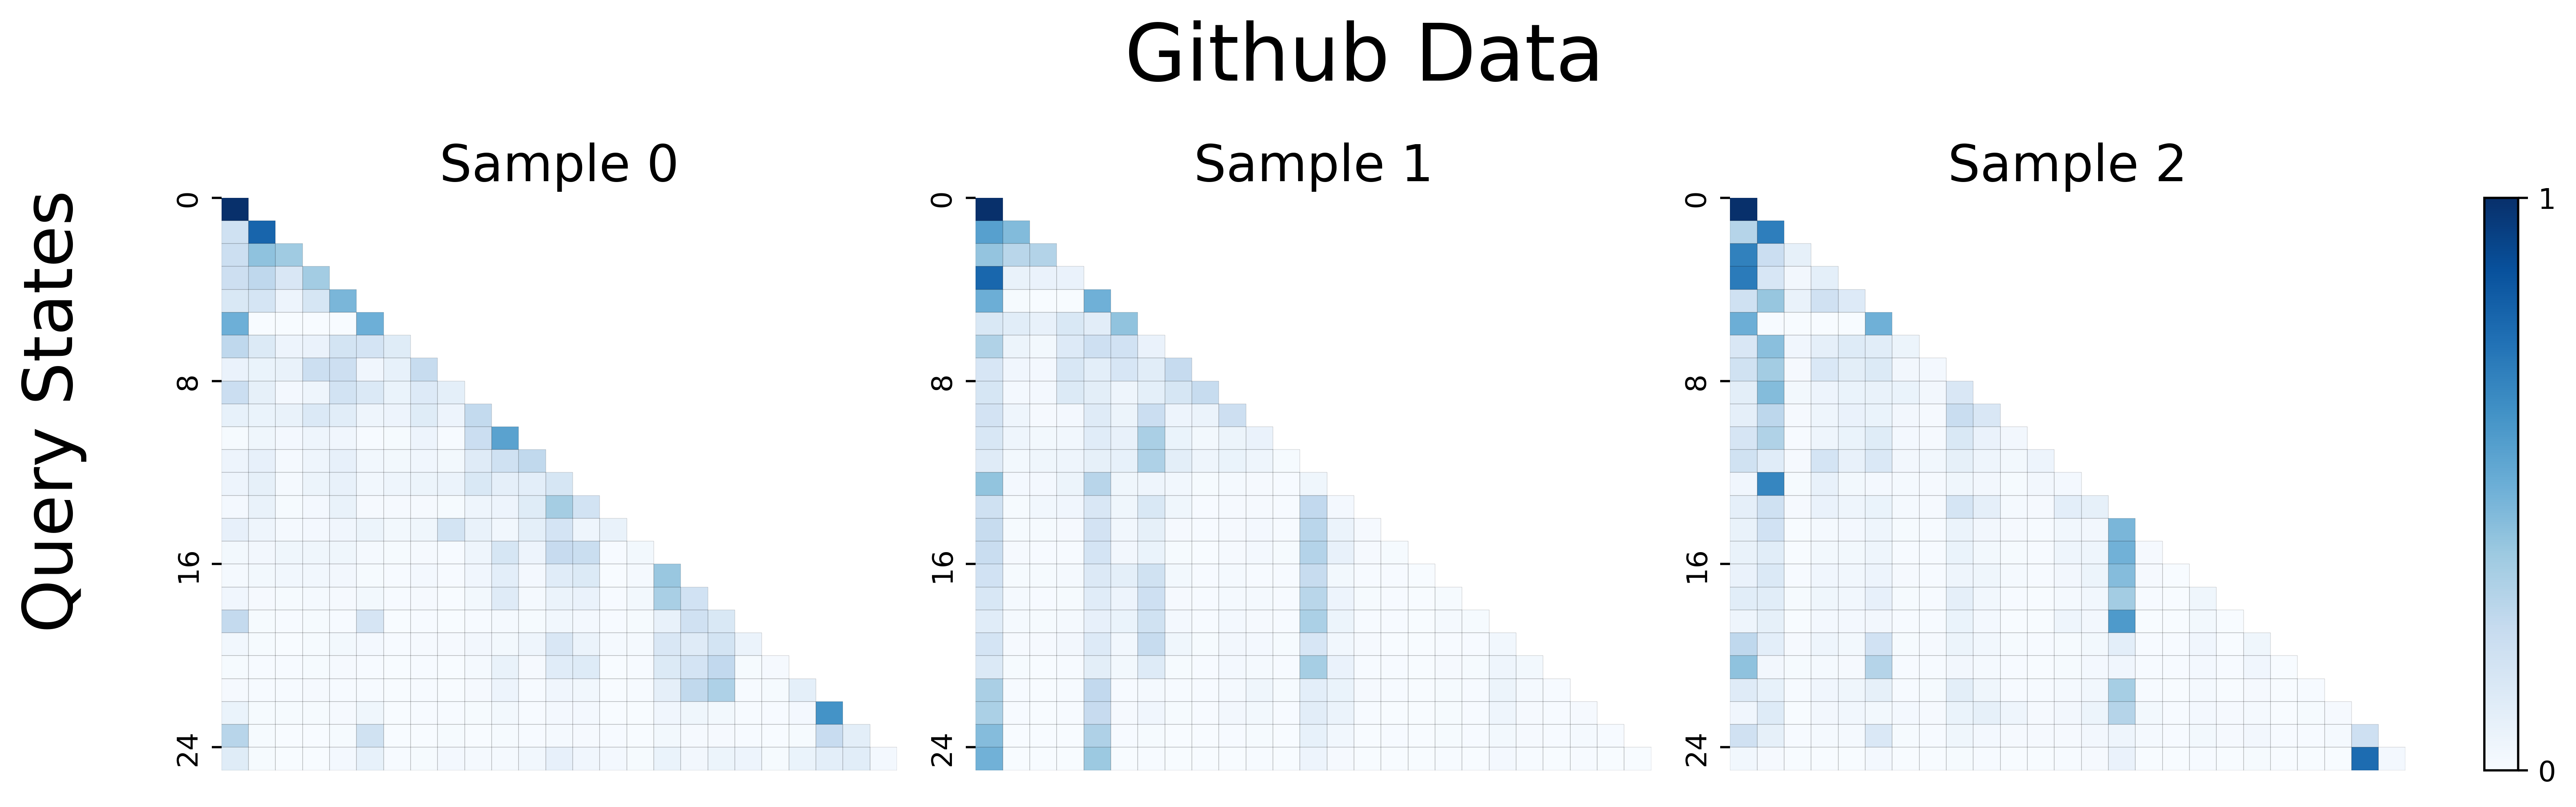
\includegraphics[width=0.9\textwidth]{Figures/L16_H25/attn_github_head25.png}
        
        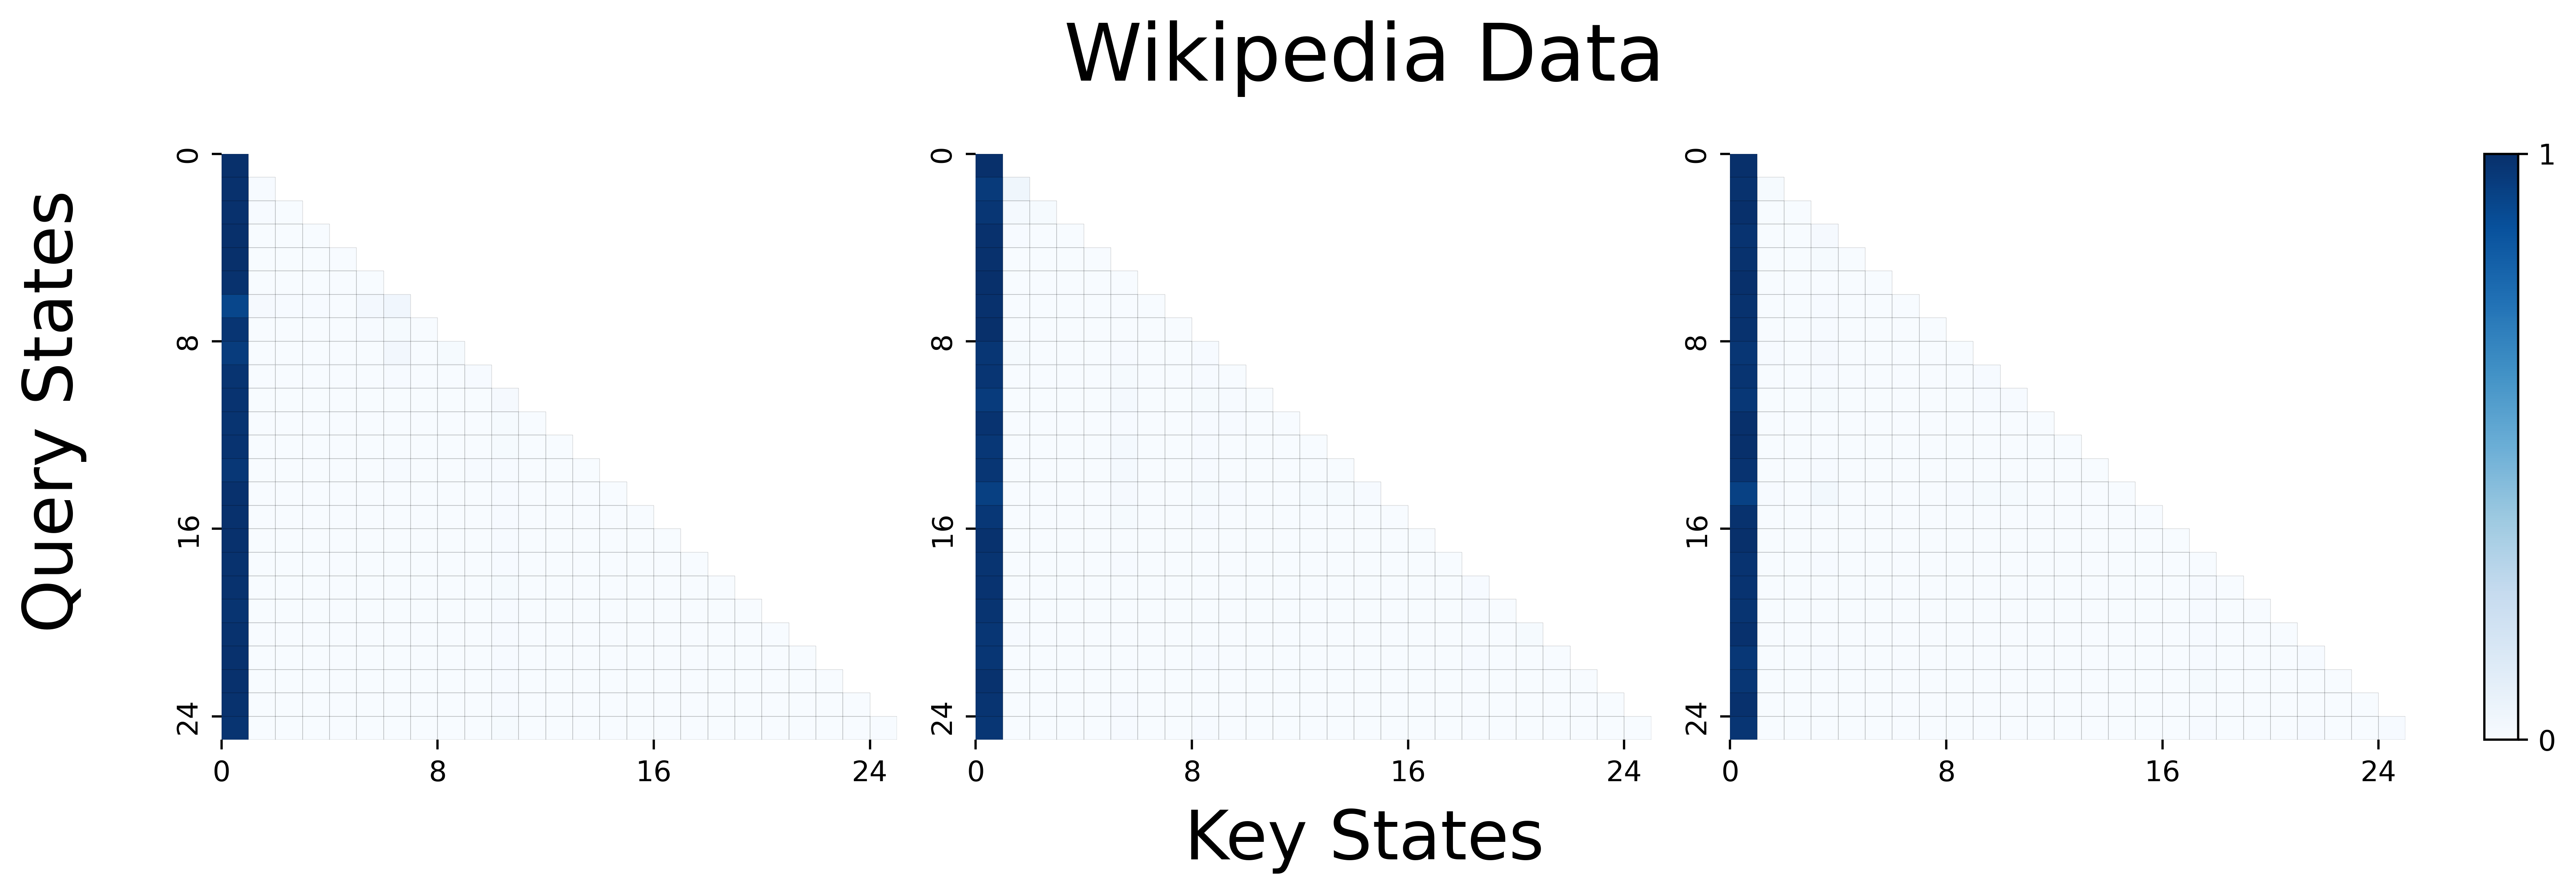
\includegraphics[width=0.9\textwidth]{Figures/L16_H25/attn_wikipedia_head25.png}
        \label{fig:github_wikipedia_weights}
    \end{subfigure}
    \hfill
    \begin{subfigure}[t]{0.38\textwidth}
        \caption{\small Zero-out-head intervention outcomes}
        \label{fig:github_wikipedia_zero_out}
        \vskip1.5em
        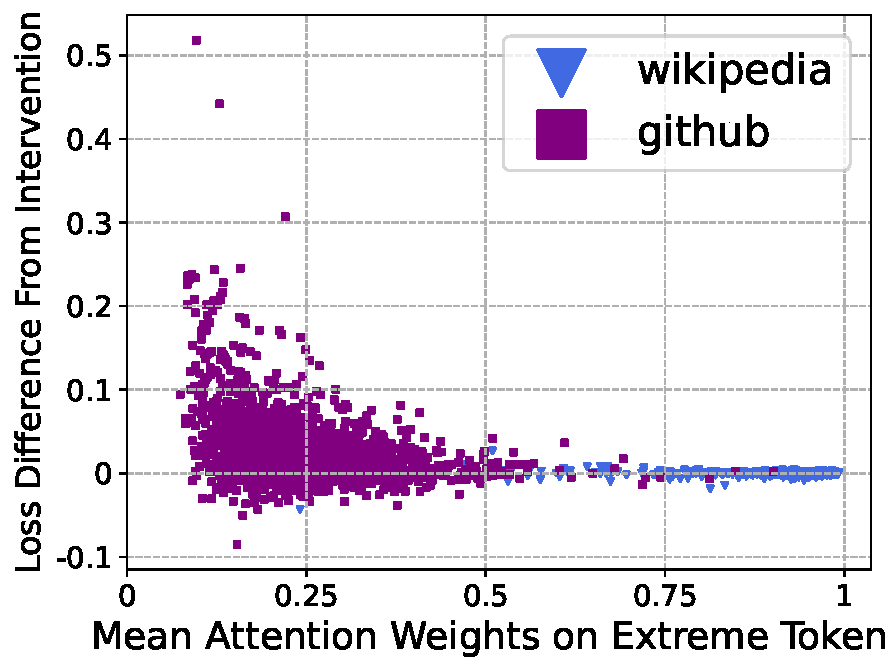
\includegraphics[width=0.9\textwidth]{Figures/BBM/LLM_interventions.pdf}
    \end{subfigure}
    \vspace{-0.5em}
    %\includegraphics[width=0.5\linewidth]{}
    \caption{\small \textbf{Active-dormant mechanism of Layer 16 Head 25 (L16H25) of Llama 2-7B-Base.} We observe that L16H25 is active on GitHub data and dormant on Wikipedia data, both sourced from RedPajama-1T \citep{together2023redpajama}. \textit{Left (a)}: Attention weights of L16H25, prompted by three randomly selected samples from each domain. \textit{Right (b)}: Results of an intervention study showing the change in cross-entropy loss when the output of L16H25 (specifically, its value states) is set to zero across sequences in both domains. The findings indicate that the model's performance for GitHub data, measured by cross-entropy loss, strongly relies on the output of this attention head. 
    % \sm{(a) Truncate at $24$ \sm{right: xlabel and xtick size. $x 0.1$} \sm{High priority} \sm{Orange color change}}
    % heads are sinks in one domain and not others (Llama 2 7B L16H25, GitHub vs Wikipedia) \DP{TODO...}
    % \DP{Plan: two figures. Left: attn sink visualization for GitHub on left and Wikipedia (4x4 (adjust to be visually appealing) samples visualize L16H25). Right: causal intervention, zeroing out head vs cross entropy delta taken across many samples from GitHub and Wikipedia.}
    }
    \label{fig:dormant_heads_domain_dependent}
\end{figure}




    %\textit{If all tokens at a head do not have helpful value states for predicting the next token, then attention mass will concentrate on tokens which are generally unhelpful for next-token prediction (like \bos). \sm{Attention heads are controlled by the active-dormant mechanism; attention sinks and value-state drains are the dormant phases of attention heads. }}

Our study of the BB model leads to the following prediction with respect to the extreme-token phenomena, which we hypothesize also applies to LLMs:  
\begin{center}
    \textit{Attention heads are controlled by an active-dormant mechanism (cf.\ Claim \ref{claim:active-dormant}). The presence of attention sinks and value-state drains indicates that an attention head is in a dormant phase.}
\end{center}

This hypothesis suggests that in LLMs, whether an attention head becomes a sink depends on the context. Specifically, the attention head may become entirely irrelevant for selecting the next tokens in certain contexts or tasks, but not in others. When this irrelevance occurs, the attention head transitions into an attention sink. This hypothesis was confirmed in small transformers and the BB task, as demonstrated in Section~\ref{sec:bb_task}. 



Accordingly, we aim to identify instances of attention heads in pretrained LLMs that exhibit this active-dormant behavior, i.e., heads that are dormant in some domains but active in others. In \Cref{fig:dormant_heads_domain_dependent}, we display a particular attention head---Layer 16 Head 25 (L16H25) of Llama 2-7B-Base \citep{touvron2023llama}---which demonstrates a clear active-dormant distinction across two distinct contexts (e.g., tokens from the GitHub subset versus the Wikipedia subset of RedPajama \citep{together2023redpajama}). While many attention heads show similar context-dependent behavior (see \Cref{sec:more_heads}), we focus on this one because the conditions for its activation are straightforward and interpretable, whereas other heads may have more nuanced criteria. 
% \sm{Can we plot more figures instead of the figures that are GitHub/Wiki}

\Cref{fig:github_wikipedia_weights} shows the attention maps of L16H25 on samples from both the GitHub and Wikipedia subsets of RedPajama. It demonstrates that L16H26 is \textit{dormant} (i.e., an attention sink) on samples from Wikipedia, which resemble prose, and \textit{active} (i.e., not an attention sink) on samples from GitHub, which resemble code. Additionally, \Cref{fig:github_wikipedia_zero_out} compares the loss difference when L16H25 is zeroed out for prompts from both domains. The results show that zeroing out this head significantly decreases model performance on GitHub sequences, while having minimal impact on Wikipedia sequences. This observation also confirms the head behaves as dormant in some contexts and active in others---in some contexts, removing this head has no effect on model performance, while in others, its removal causes significant performance drops.
% We include more detail in \Cref{sec:circuit}.
% , where we extract a circuit for extreme-token phenomena to examine the dormant-active mechanism and its interaction with input token semantics. \sm{Polish} \sm{Mid priority}



% Accordingly, we strive to find instances of heads in pretrained LLMs that satisfy this principle, i.e., which are dormant on some domains and active on others. In \Cref{fig:dormant_heads_domain_dependent}, we show a particular attention head -- Layer 16 Head 25 of Llama 2-7B-Base \citep{touvron2023llama} --- which has an extremely clear active-dormant distinction across two distinct contexts (e.g., tokens from RedPajama \citep{together2023redpajama} drawn from the GitHub subset versus the Wikipedia subset). While there are many such attention heads which are context-dependent --- we provide some in \Cref{sec:more_heads} --- we demonstrate this one because the conditions under which it is active are simple and interpretable, while others have more involved or complex criteria to become active. We observe that this attention head is \textit{dormant} (i.e., an attention sink) on samples from Wikipedia, which more closely resemble prose, and \textit{active} (i.e., not an attention sink) on samples from GitHub, which more closely resemble code. We also observe that this attention head, in general, contributes significantly to the performance of the model on code sequences, but has negligible impact on the performance of the model on prose sequences (\Cref{fig:github_wikipedia_zero_out}). This is a further justification, from a practical perspective, of why this head is sometimes dormant and sometimes active --- in some contexts we can ablate it from the model entirely with no effect, but in other contexts ablating the head leads to huge performance drops. We include more detail in \Cref{sec:circuit}, where we extract a circuit for extreme-token phenomena in order to analyze the dormant-active mechanism and its interaction with the semantics of the input tokens.

%\footnote{Llama 2-7B-Base has two sink tokens (\bos~and one more) in its attention sink heads, while Llama 3.1-8B-Base only has one (\bos). We discuss a potential reason in \Cref{sub:multiple_sinks_discussion}. \sm{Why we put this remark here?}} \sm{Talk about other heads also has dormant and active phase, though not interpretable. Ablation figures in appendix. } \DP{@SM: the first part is already in the paragraph.} \sm{It would be good to link to figures for other heads. } \DP{sure will add to appendix, and comment out this comments when done}

\subsection{Extreme-token phenomena along training dynamics of LLMs}\label{sub:olmo_dynamics}


\begin{figure}[t]
    \centering
    \begin{subfigure}[t]{0.32\textwidth}
        \centering 
        \caption{\small Attention sink dynamics}
        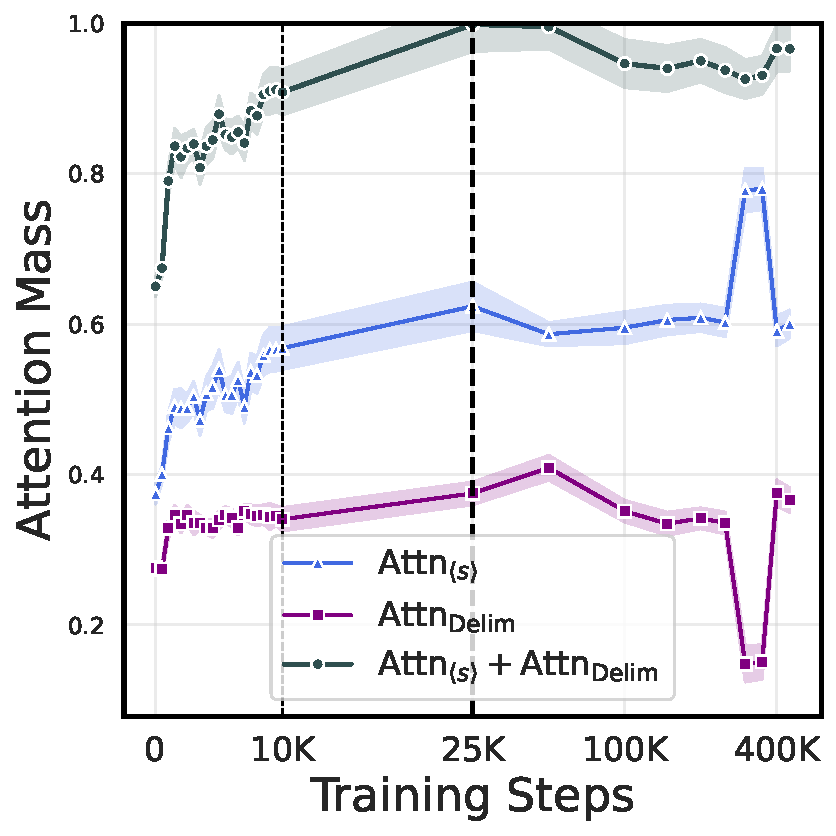
\includegraphics[width=0.9\textwidth]{Figures/olmo/attn_mass_on_top_two_tokens.pdf}
        \label{fig:olmo_sink}
    \end{subfigure}
    \begin{subfigure}[t]{0.32\textwidth}
        \centering 
        \caption{\small Value state dynamics}
        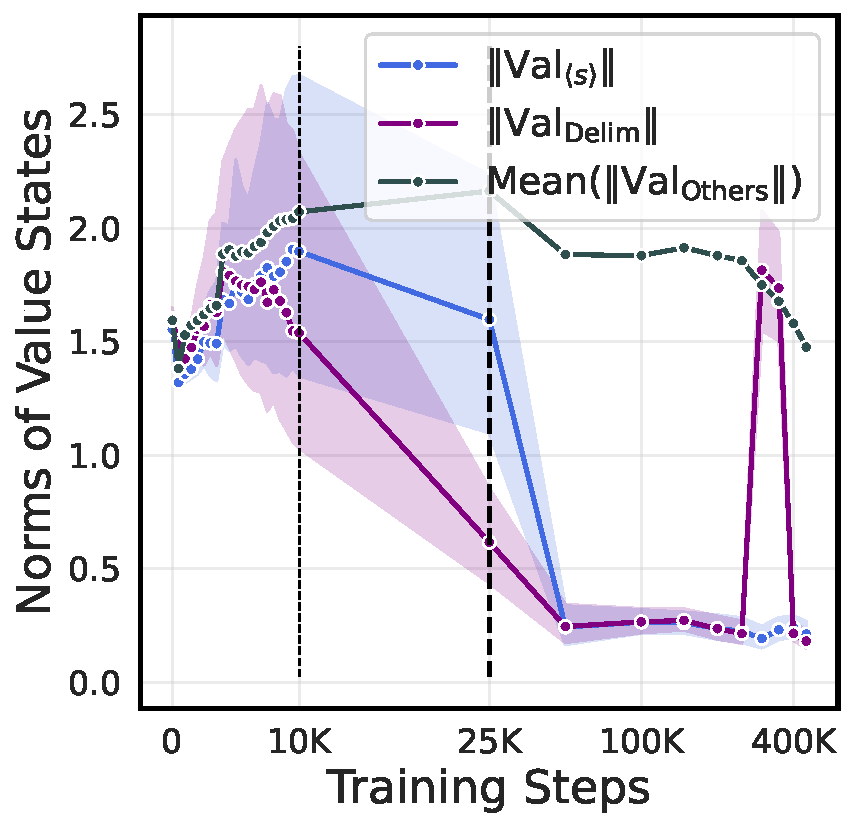
\includegraphics[width=0.9\textwidth]{Figures/olmo/value_norms.pdf}
        \label{fig:olmo_drain}
    \end{subfigure}
    \begin{subfigure}[t]{0.32\textwidth}
        \centering 
        \caption{\small Residual state dynamics}
        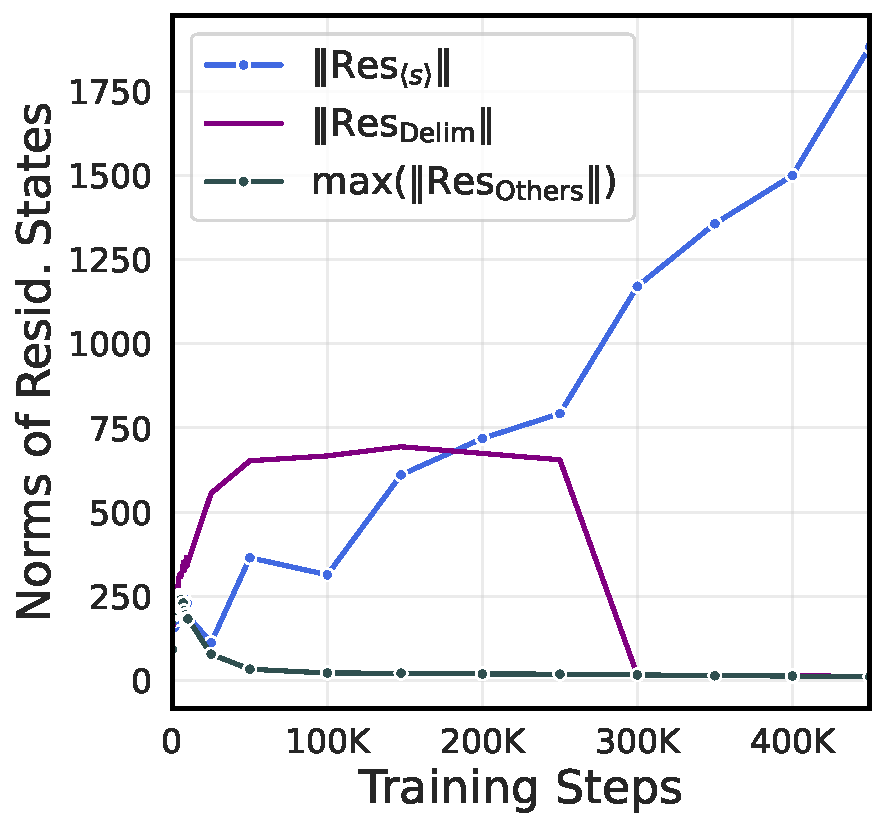
\includegraphics[width=0.9\textwidth]{Figures/olmo/layer_output_norms.pdf}
        \label{fig:olmo_peak}
    \end{subfigure}
    % \vspace{-2em}
    \caption{\small \textbf{Attention weights, value state norms, and residual state norms of Layer 24 during the training dynamics of OLMo.} \textit{Left (a)}: The total attention mass on extreme tokens \bos~and ``\text{Delim}''(\period) at Layer 24, averaged across all attention heads. The horizontal axis is logarithmically scaled after step $10$k. We observe a rapid increase followed by stabilization within the range \([0.9, 1]\) for the rest of training, consistent with our predictions. \textit{Middle (b)}: The value state norms of each token at Layer 24 during training, averaged over all heads. The horizontal axis is logarithmically scaled after step $10k$. Initially, the value states of all tokens shrink, eventually converging, while the value states of the extreme tokens shrink to significantly lower levels compared to other tokens. Figure \textit{(a)} and \textit{(b)} coincide with the trends in Figure~\ref{fig:dynamics} under the BB task. \textit{Right (c)}: The residual state norms of each token at Layer 24 during training. The residual state norm of \bos~increases linearly in magnitude throughout training, matching Figure~\ref{fig:sgd} in the BB task.}
    % \sm{Thicker} \sm{L24 is a bit repetitive} \sm{For (a) and (b), is there a way to draw 0 - 50K using linear scale and 50K - 500K using log scale? This could match better Figure 3(b)} \tianyu{link back to corresponding figures in BB task}}



    
    \label{fig:olmo_predictions_phase0}
\end{figure}
\begin{figure}[h]
    \centering
    \hfill
    \begin{subfigure}[t]{0.32\textwidth}
        \centering 
        \caption{\small Logit dynamics}
        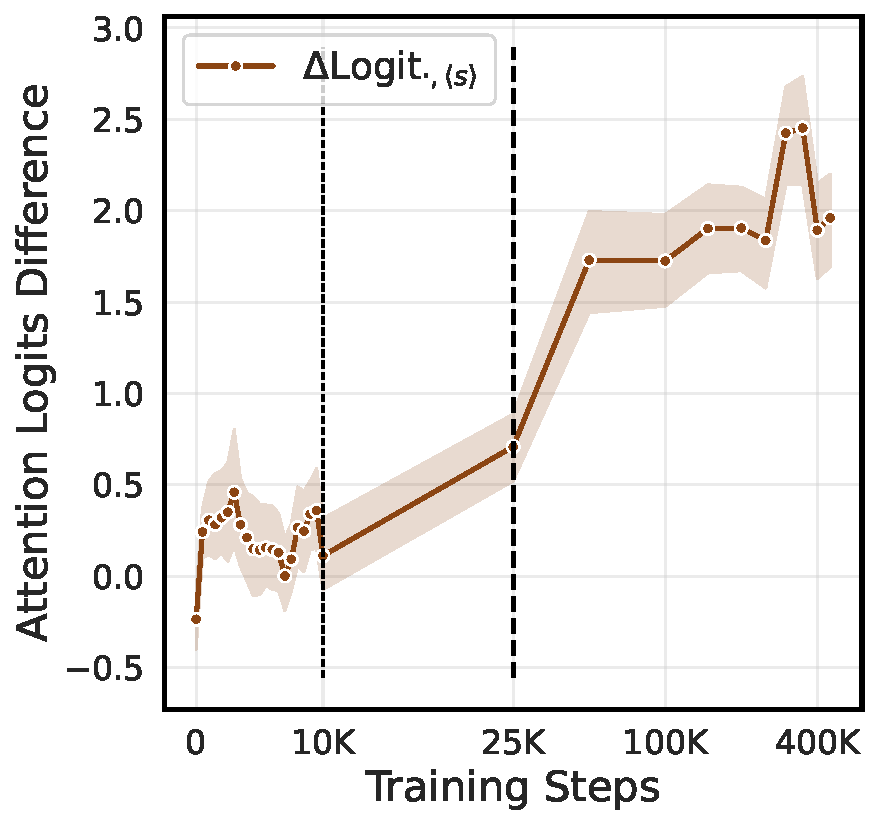
\includegraphics[width=0.9\textwidth]{Figures/olmo/attention_logits.pdf}
        \label{fig:attention_logits_olmo_dynamic}
    \end{subfigure}
    \hfill
    \begin{subfigure}[t]{0.32\textwidth}
        \centering 
        \caption{\small Sink-logits concentration}
        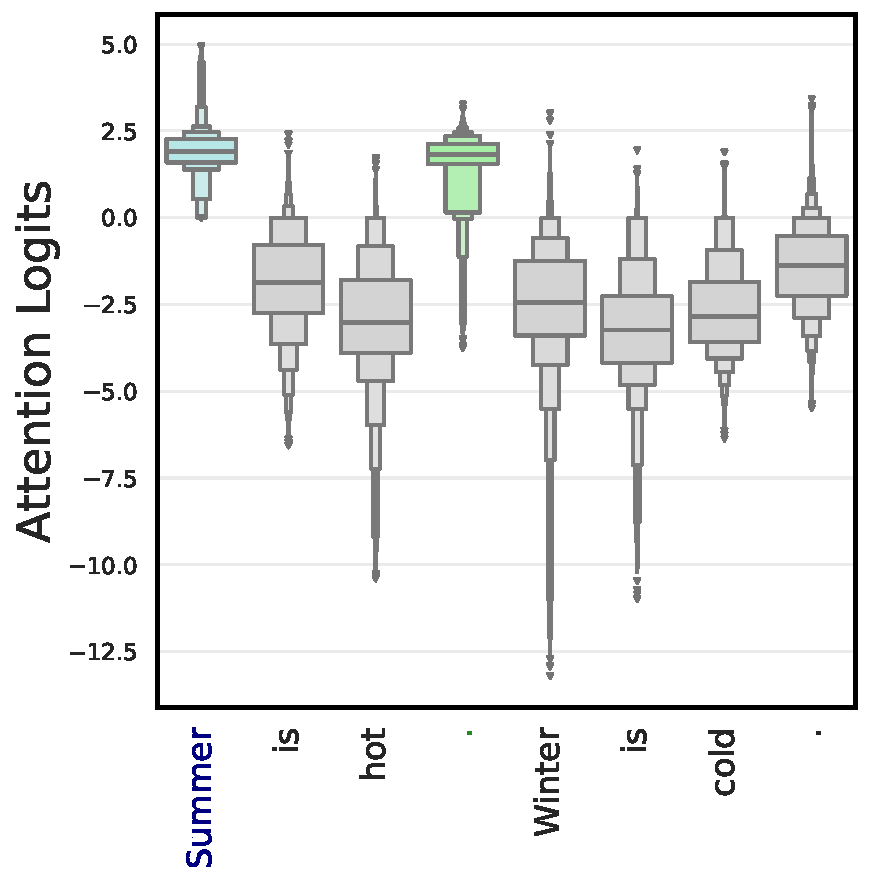
\includegraphics[width=0.9\textwidth]{Figures/olmo/attention_logits_on_test.pdf}
        \label{fig:attention_logits_olmo_static}
    \end{subfigure}
    \hfill
    \phantom{.}
    % \vspace{-2em}
        \caption{\small \textbf{Attention logits of Layer 24.}  \textit{Left (a)}: Attention logits difference of all tokens' query states against \bos's key state during training. The difference in attention logits is computed as \(\Delta\mathrm{logit}_{\cdot,\bos} = \query_{\cdot}^\top \key_{\bos} - \text{Mean}[\query_{\cdot}^\top \key_{\text{Others}}]\). The horizontal axis is logarithmically scaled after step $10k$. We observe that $\Delta \mathrm{logit}_{\cdot,\bos}$ increases approximately in logarithmic scale during training steps $10$k to $100$k, matching the decreasing phase of the value states in Figure~\ref{fig:olmo_drain}. 
        % This behavior aligns with the stable-phase prediction made in the BB model in \Cref{thm:main}(c). Note that this prediction does not apply to the logit corresponding to the zeroth query and key token, as its softmax value will be set to \(1\), making its behavior irrelevant for prediction. 
        \textit{Right (b)}: Attention logits of the last token's query state against all token's key states for pretrained OLMo. In this experiment, we generate \(128\) randomly sampled test tokens with IDs from \(100\) to \(50000\) in the OLMo tokenizer. We append each token separately to the test phrase ``Summer is warm\period~Winter is cold\period'', creating \(128\) different samples, which we feed to the LLM to examine the model behavior. We plot the distribution of (un-shifted) attention logits \( \text{logit}_{\cdot,\tok}=\query_{\mathrm{test}}^\top \key_{\tok}\) across all heads at Layer 24 and all test tokens. The distribution of $\text{logit}_{\cdot,\bos}$ and $\text{logit}_{\cdot,\text{Delim}}$ have considerably small variance compared with other logits, confirming the sink-logits concentration phenomenon. }
        % \tianyu{maybe to make it more clear, we can say that the variance of the attention logits on \bos~is small. Or we can use a new name (attention logits concentration)} \sm{tick size. Box thicker. } \sm{pdf} \tianyu{change the logit in (a)}}
    % \caption{\small \textbf{Attention logits of Layer 24.}  \textit{Left (a)}: The normalized attention logits of all tokens' query states against \bos's key state during training \sm{Is it the opposite?}. We observe that the logits of all non-extreme tokens' query states against \bos's key state in OLMo's Layer 24 are stable for a large fraction of the training run, after an initialization period. This echoes the stable phase prediction made in the BB model in \Cref{thm:main}(c). Note that this prediction makes no guarantees about the logit corresponding to the zeroth query token and zeroth key token, which will be set to \(1\) by the softmax and so its behavior is irrelevant for prediction. Also note that we use normalization, similar to \Cref{sec:bb_task}, to make all terms comparable; namely we have \(\mathrm{logit}_{i} = \langle \query_{i}, \key_{0}\rangle - \mathtt{mean}_{j}(\langle \query_{i}, \key_{j}\rangle)\). \textit{Right (b)}: \sm{A summary phrase of the figure.} For this experiment, we generate \(128\) randomly sampled test tokens with IDs from \(100\) to \(50000\) in the OLMo tokenizer. We append each token separately to the test phrase ``Summer is warm. Winter is cold.'', creating \(128\) different samples, which we feed to the LLM to record the model behavior. We plot the distribution of (un-normalized) dot products \(\langle \query_{\mathrm{test}}, \key_{j}\rangle\) across all heads at Layer 24 and all test tokens. We observe that logits of all regular tokens have very similar distributions, and the distributions of the logits corresponding to extreme tokens \(0\) and \(3\) are also similar. \sm{Why similar? } This confirms the hypothesis that at the end of training, attention heads converge to the stable phase, with similar logits on extreme tokens. \tianyu{maybe to make it more clear, we can say that the variance of the attention logits on \bos~is small. Or we can use a new name (attention logits concentration)} \sm{tick size. Box thicker. } }
    \label{fig:olmo_predictions_phase1}
\end{figure}


Our study of the BB model leads to the following prediction about the dynamical behavior of the extreme-token phenomena, which we hypothesize also applies to LLMs:  
\begin{center}
    \textit{Attention heads undergo an attention-increasing and value-state-shrinking phase driven by the mutual reinforcement mechanism (cf.\ Claim~\ref{claim:mutual-reinforcement}). This is followed by a stable phase, where all non-trigger tokens have large, nearly identical attention logits on the extreme token. Simultaneously, the residual state norms of the extreme tokens increase linearly during pretraining.}
\end{center}



% We confirm these predictions below, thus demonstrating the overall validity of the BB task as a model for extreme token phenomena in LLMs. 
We confirm these predictions below. To observe the training dynamics of a large-scale LLM, we use the setup of OLMo-7B-0424 \citep{groeneveld2024olmo} (henceforth just referred to as OLMo), which provides open-sourced weights at various stages of their training.\footnote{We did not analyze Llama for dynamics, as they do not provide open-source intermediate checkpoints along pretraining.} For our analysis, we inspect OLMo at multiple checkpoints: every 500 steps for the first 10,000 steps, then at 25,000 steps, 50,000 steps, and every 50,000 steps up to 449,000 steps (approximately the end of their training).\footnote{For the single 150,000-step checkpoint, we observed that its statistics were outliers, which we hypothesize is due to a system failure. We address this by using the average of nearby checkpoints to represent its statistics.} The input we use for this analysis is again ``Summer is warm\period~Winter is cold\period''\footnote{Note that OLMo does not have a \bos~token, but attention sinks still form in the majority of heads. In particular, the first token always behaves as an attention sink. We discuss this further in \Cref{sub:fixed_bos}.} In this prompt, the ``$\mathrm{Delim}$'' token, namely ``\period'', also becomes a sink token along with \bos. We believe this occurs because the period is not semantically meaningful and is not useful for predicting future tokens (cf.\  \Cref{sub:fixed_bos}) 
% \sm{Footnote 4 could be made as part of the main text}


% \tianyu{revise the mutual reinforcement mech part}
\Cref{fig:olmo_predictions_phase0} illustrates the dynamics of attention weights, value state norms, and the residual state norms for attention heads in Layer 24 of OLMo. The figure shows that the average attention on extreme tokens (\bos~and $\mathrm{Delim}$) increases rapidly at the beginning of training before stablizing, while the value state norms of these extreme tokens decrease during training steps 10k-100k. The synchronized evolution of attention weights and value state norms aligns with the prediction of the mutual reinforcement mechanism.  Additionally, the residual states of \bos~increase linearly, while those of other tokens converge to a small number. \Cref{fig:olmo_predictions_phase1} provides a more detailed examination of the attention logits in Layer 24 of OLMo. Figure~\ref{fig:attention_logits_olmo_dynamic} presents the dynamics of the difference in attention logits, showing that $\Delta \text{logit}_{\cdot,\bos}$ increase during training steps 10k-100k, matching the decreasing phase of the value states.
Figure~\ref{fig:attention_logits_olmo_static} also demonstrates the \textit{sink-logits concentration} phenomenon. Specifically, it shows that the sink logits will eventually converge to a stable phase, in which logits corresponding to the key of the sink token and queries of all non-sink tokens are nearly identical. These findings coincide with the dynamical behavior predicted by the BB model, as outlined in Theorem~\ref{thm:main}(c) and corroborated by the experimental results in \Cref{figure:verify-assumptions}. 

% with the attention logits corresponding to \bos's key and other token's query converging to near identical value \sm{Name for this logit}
% In \Cref{fig:olmo_predictions_phase0}, we confirm that attention heads go through an attention-increasing and value-state-shrinking phase, and that the residual state norm of the \bos{} token increases linearly during pretraining. We show that, at Layer 24 of OLMo, the average attention on extreme tokens (\bos~and $\mathrm{Delim}$) increases rapidly at the beginning of training and converges to a constant, while the value state norms of extreme tokens decrease rapidly. Also, the residual states of extreme tokens also increase linearly, while the rest quickly converge. In \Cref{fig:olmo_predictions_phase1} we show that attention heads converge to a stable phase, and that all logits corresponding to the first token's value states (i.e., all tokens' value of \(\mathrm{logit}_{0}\), except possibly the value of \(\mathrm{logit}_{0}\) corresponding to \bos~itself) have similar distributions. These confirm our dynamics insights from the BB model (cf.\ \Cref{figure:verify-assumptions}). 

%\sm{These echos the findings from the BB model. Link figure 3b here. }
% Outline:
% \begin{itemize}
%     \item OLMo value states at a middle layer are roughly constant over time except for bos token and first delimiter
%     \item Massive norm keeps increasing over time 
%     \item Attention sink occurs very rapidly and stays constant over time
% \end{itemize}

% \begin{figure}
%     \centering
%     %\includegraphics[width=0.5\linewidth]{}
%     \caption{Training dynamics of value states, massive norm, and attention sink via OLMo
%     \DP{TODO: for attention logits plot, put linear plot for first 10k epochs (halfway through axis) and log plot for remaining epochs; do the same for value states; plot multiple heads for value plot}}
%     \label{fig:enter-label}
% \end{figure}












